\subsubsection{Назначение вкладки МКО}

Вкладка МКО предназначена для проверки функций микросервиса МКО через графический интерфейс рабочего места оператора. Она позволяет задавать параметры работы модуля МКО, вызывать команды драйвера, получать результаты обмена, работать со словами данных и контролировать ход выполнения операций по журналу.

Вкладка разделена на две основные части:

\begin{itemize}
	\item левая часть используется для работы в режиме КК, то есть в режиме контроллера канала;
	\item правая часть используется для работы в режиме ОУ, то есть в режиме оконечного устройства.
\end{itemize}

Режим КК предназначен для настройки контроллера канала, задания параметров обмена, запуска обмена и получения результатов. Режим ОУ предназначен для настройки оконечного устройства, чтения и записи подадресов, изменения ответного слова, очистки буферов и получения входящих команд.

\begin{figure}[H]
	\centering
	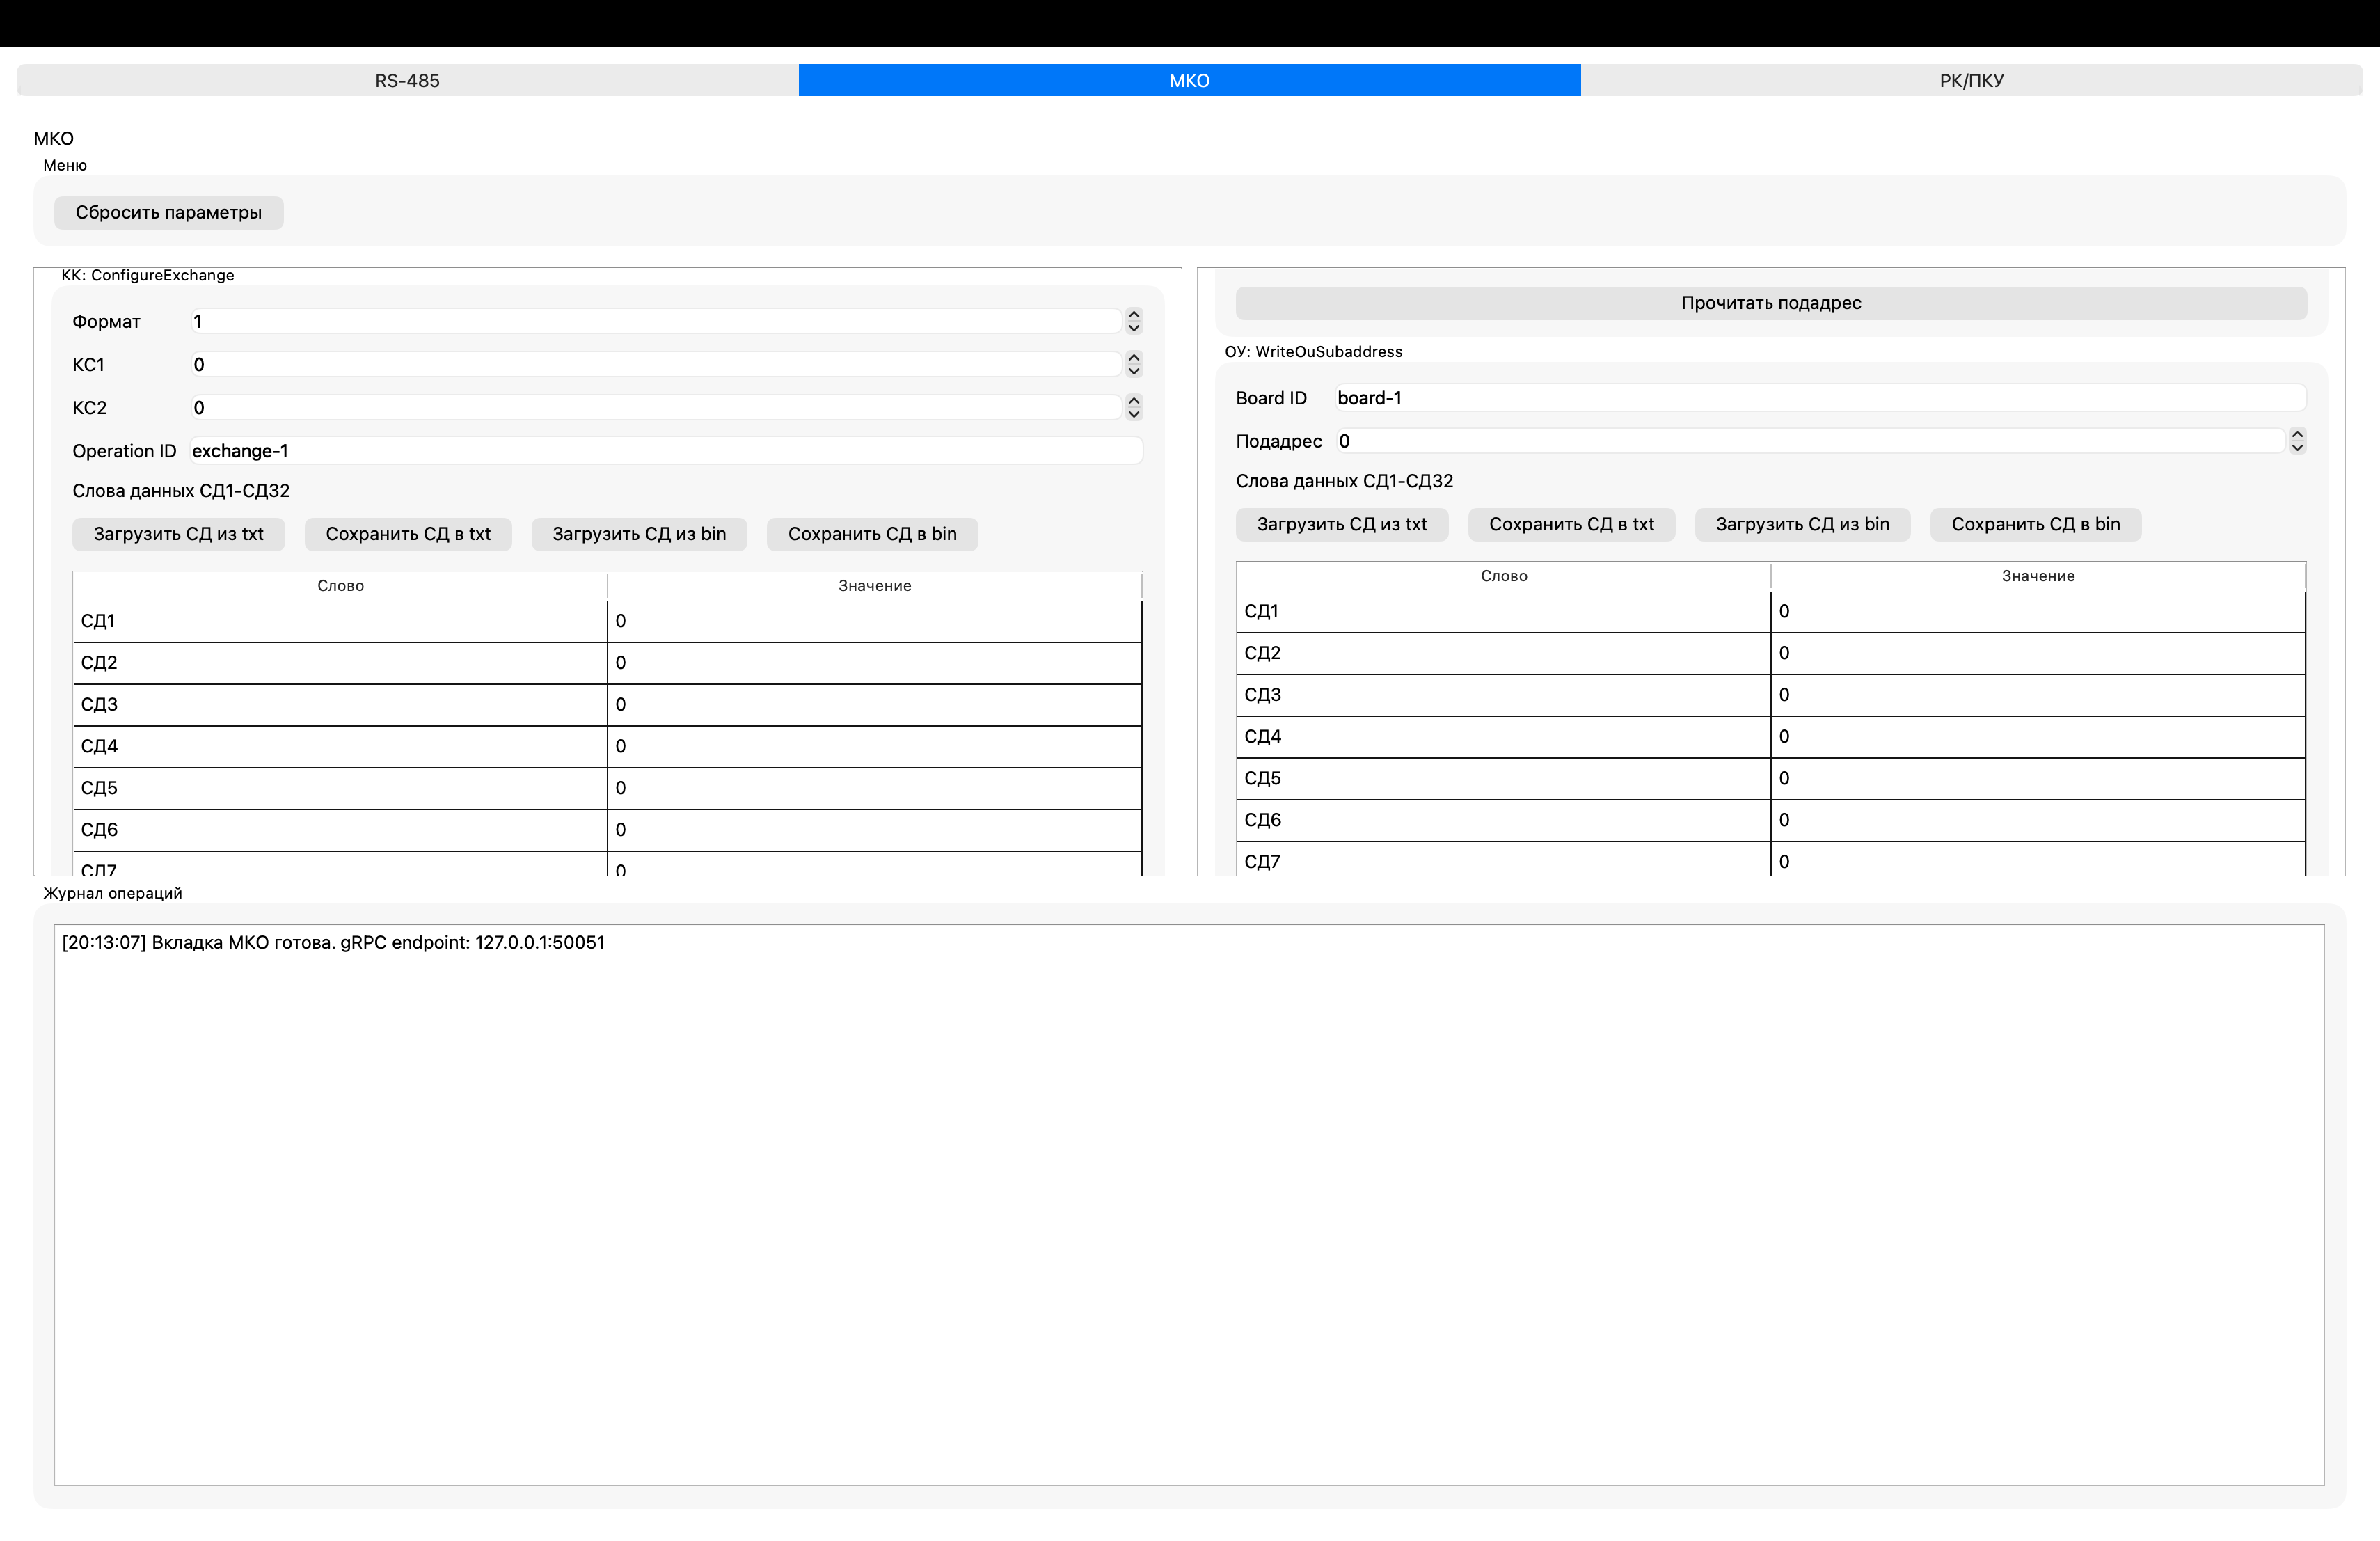
\includegraphics[width=\textwidth]{mko/image.png}
	\caption{Общий вид вкладки МКО}
\end{figure}

\begin{figure}[H]
	\centering
	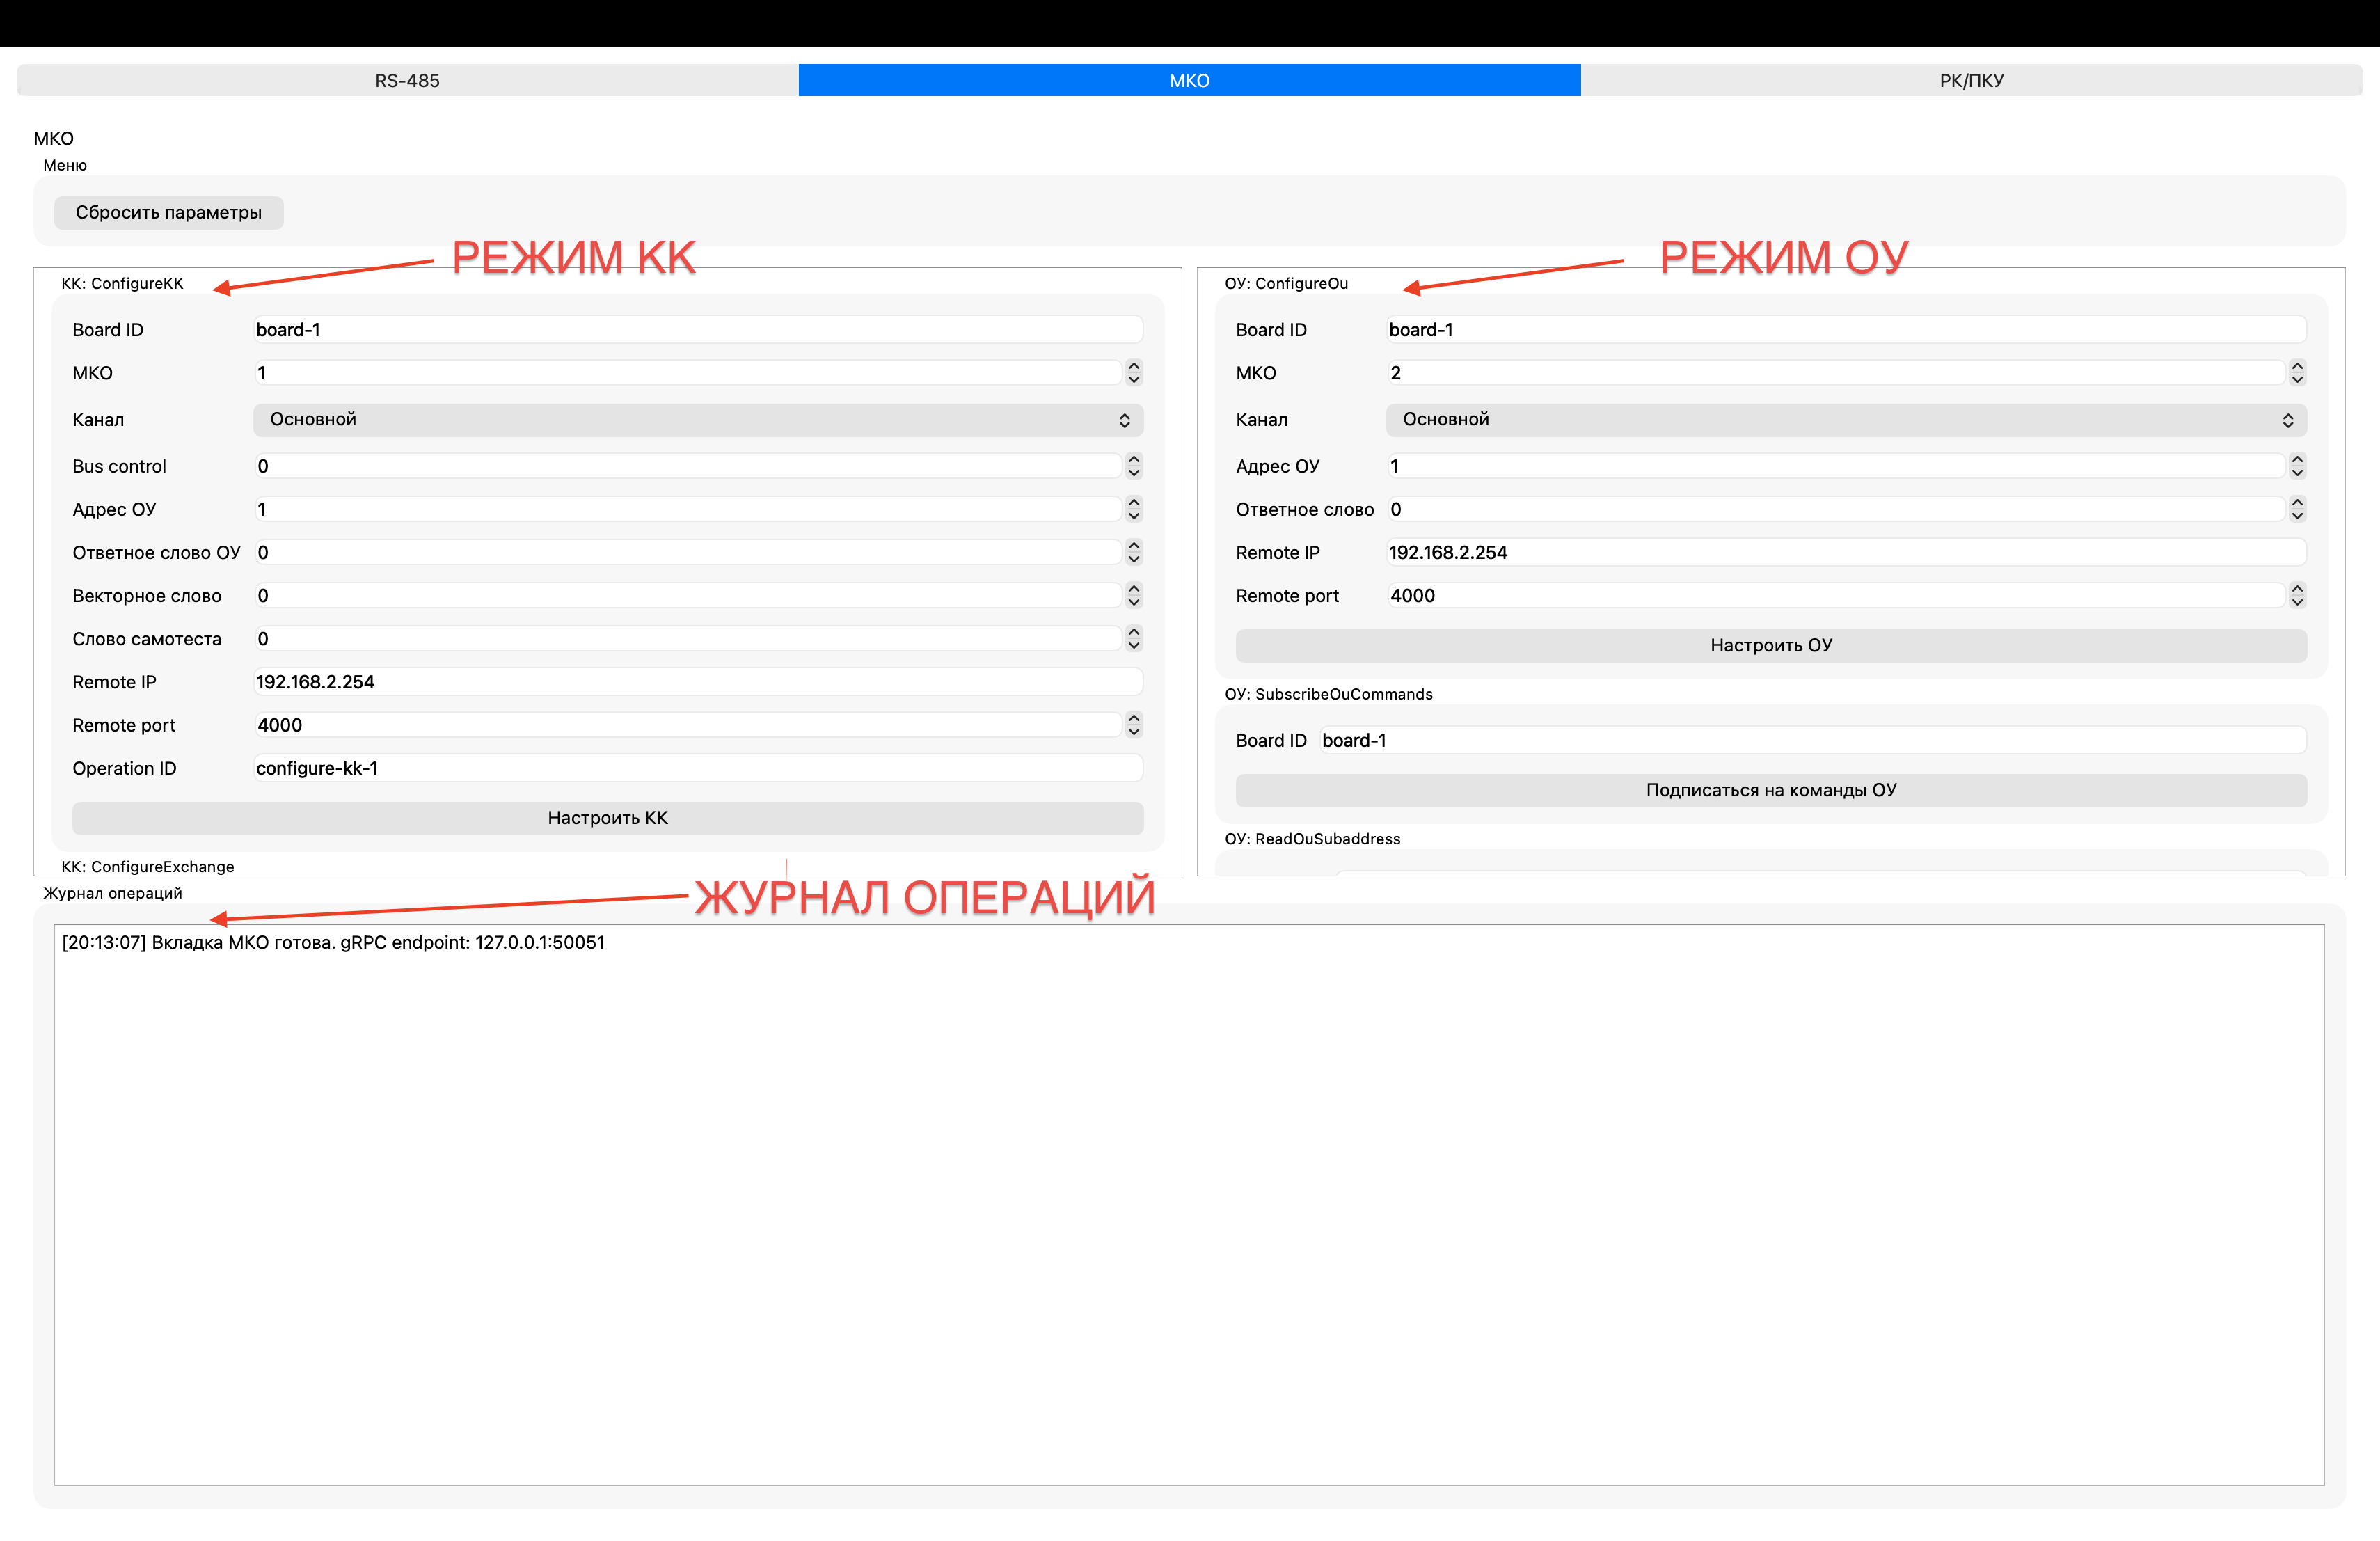
\includegraphics[width=\textwidth]{mko/image-1.png}
	\caption{Подсказки основных блоков вкладки МКО}
\end{figure}

\subsubsection{Условия работы вкладки МКО}

Для работы вкладки МКО должны быть запущены графический интерфейс, микросервис МКО и драйвер МКО. Для локальной проверки вместо реального драйвера допускается использовать заглушку драйвера \texttt{fake-mko-driver}.

При работе с реальным оборудованием должна быть доступна плата МКО, а в параметрах настройки должен быть указан ее сетевой адрес и порт. При работе через заглушку используются адрес и порт запущенного отладочного драйвера.

\subsubsection{Локальное развертывание для проверки}

Для проверки без реальной платы используется цепочка:

\begin{center}
	\texttt{GUI -> микросервис МКО -> fake-mko-driver}
\end{center}

Перед запуском необходимо проверить файл локальной конфигурации:

\begin{center}
	\texttt{mko/config/local.env}
\end{center}

В нем должны быть заданы адрес микросервиса МКО и адрес драйвера:

\begin{lstlisting}[language=bash]
export MKO_SERVICE_ADDR=127.0.0.1:50051
export MKO_DRIVER_ADDR=127.0.0.1:50052
\end{lstlisting}

Параметр \texttt{MKO\_SERVICE\_ADDR} задает адрес, на котором микросервис МКО принимает gRPC-вызовы от графического интерфейса. Параметр \texttt{MKO\_DRIVER\_ADDR} задает адрес, по которому микросервис обращается к драйверу МКО. При локальной проверке по этому адресу запускается \texttt{fake-mko-driver}.

Локальный запуск выполняется в следующем порядке:

\begin{enumerate}
	\item открыть первый терминал и перейти в каталог микросервиса:
\begin{lstlisting}[language=bash]
cd practice2026/mko
\end{lstlisting}

	\item запустить заглушку драйвера:
\begin{lstlisting}[language=bash]
go run ./cmd/fake-mko-driver
\end{lstlisting}

	После запуска должно появиться сообщение о прослушивании порта \texttt{50052};

	\item открыть второй терминал и перейти в каталог микросервиса:
\begin{lstlisting}[language=bash]
cd practice2026/mko
\end{lstlisting}

	\item загрузить локальные переменные окружения:
\begin{lstlisting}[language=bash]
source config/local.env
\end{lstlisting}

	\item запустить микросервис МКО:
\begin{lstlisting}[language=bash]
go run ./cmd/mko-service
\end{lstlisting}

	Микросервис должен принимать вызовы графического интерфейса по адресу \texttt{127.0.0.1:50051} и обращаться к \texttt{fake-mko-driver} по адресу \texttt{127.0.0.1:50052};

	\item открыть третий терминал и запустить графический интерфейс:
\begin{lstlisting}[language=bash]
cd practice2026/gui/src
./build.sh
./build/out/ui.app/Contents/MacOS/ui
\end{lstlisting}

	Если графический интерфейс уже собран, повторная сборка не требуется. В этом случае достаточно запустить исполняемый файл;

	\item открыть вкладку МКО и проверить журнал операций. В журнале должно появиться сообщение о готовности вкладки и адресе \texttt{127.0.0.1:50051}.
\end{enumerate}

Если порт \texttt{50052} занят, необходимо остановить ранее запущенный процесс \texttt{fake-mko-driver} или изменить порт в настройках запуска и в файле \texttt{local.env}. Если порт \texttt{50051} занят, необходимо освободить его или изменить значение \texttt{MKO\_SERVICE\_ADDR} и адрес подключения графического интерфейса.

\subsubsection{Правила ввода значений}

Числовые поля вводятся в соответствии с диапазонами, которые ожидает драйвер и контракт микросервиса. Для слов данных СД допускается ввод как в десятичной, так и в шестнадцатеричной системе счисления. Например, значения \texttt{4660} и \texttt{0x1234} интерпретируются одинаково.

При загрузке слов данных из текстового файла допускаются строки следующих видов: \texttt{0x1234}, \texttt{4660}, \texttt{SD1=0x1234}, \texttt{1 0x1234}. Допускается использовать русское обозначение СД в файле, однако для переносимости рекомендуется использовать латинское обозначение \texttt{SD}.

В строке может быть комментарий после символа \texttt{\#} или последовательности \texttt{//}. Пустые строки игнорируются. Из файла загружается не более 32 слов. Если слов меньше 32, оставшиеся строки таблицы заполняются нулями.

Для двоичных файлов используется формат \texttt{uint32 little-endian}: одно слово СД занимает 4 байта. При импорте из двоичного файла читается не более 32 слов. Если размер файла не кратен 4 байтам, неполный хвост игнорируется, а сообщение об этом выводится в журнал операций.

\begin{figure}[H]
	\centering
	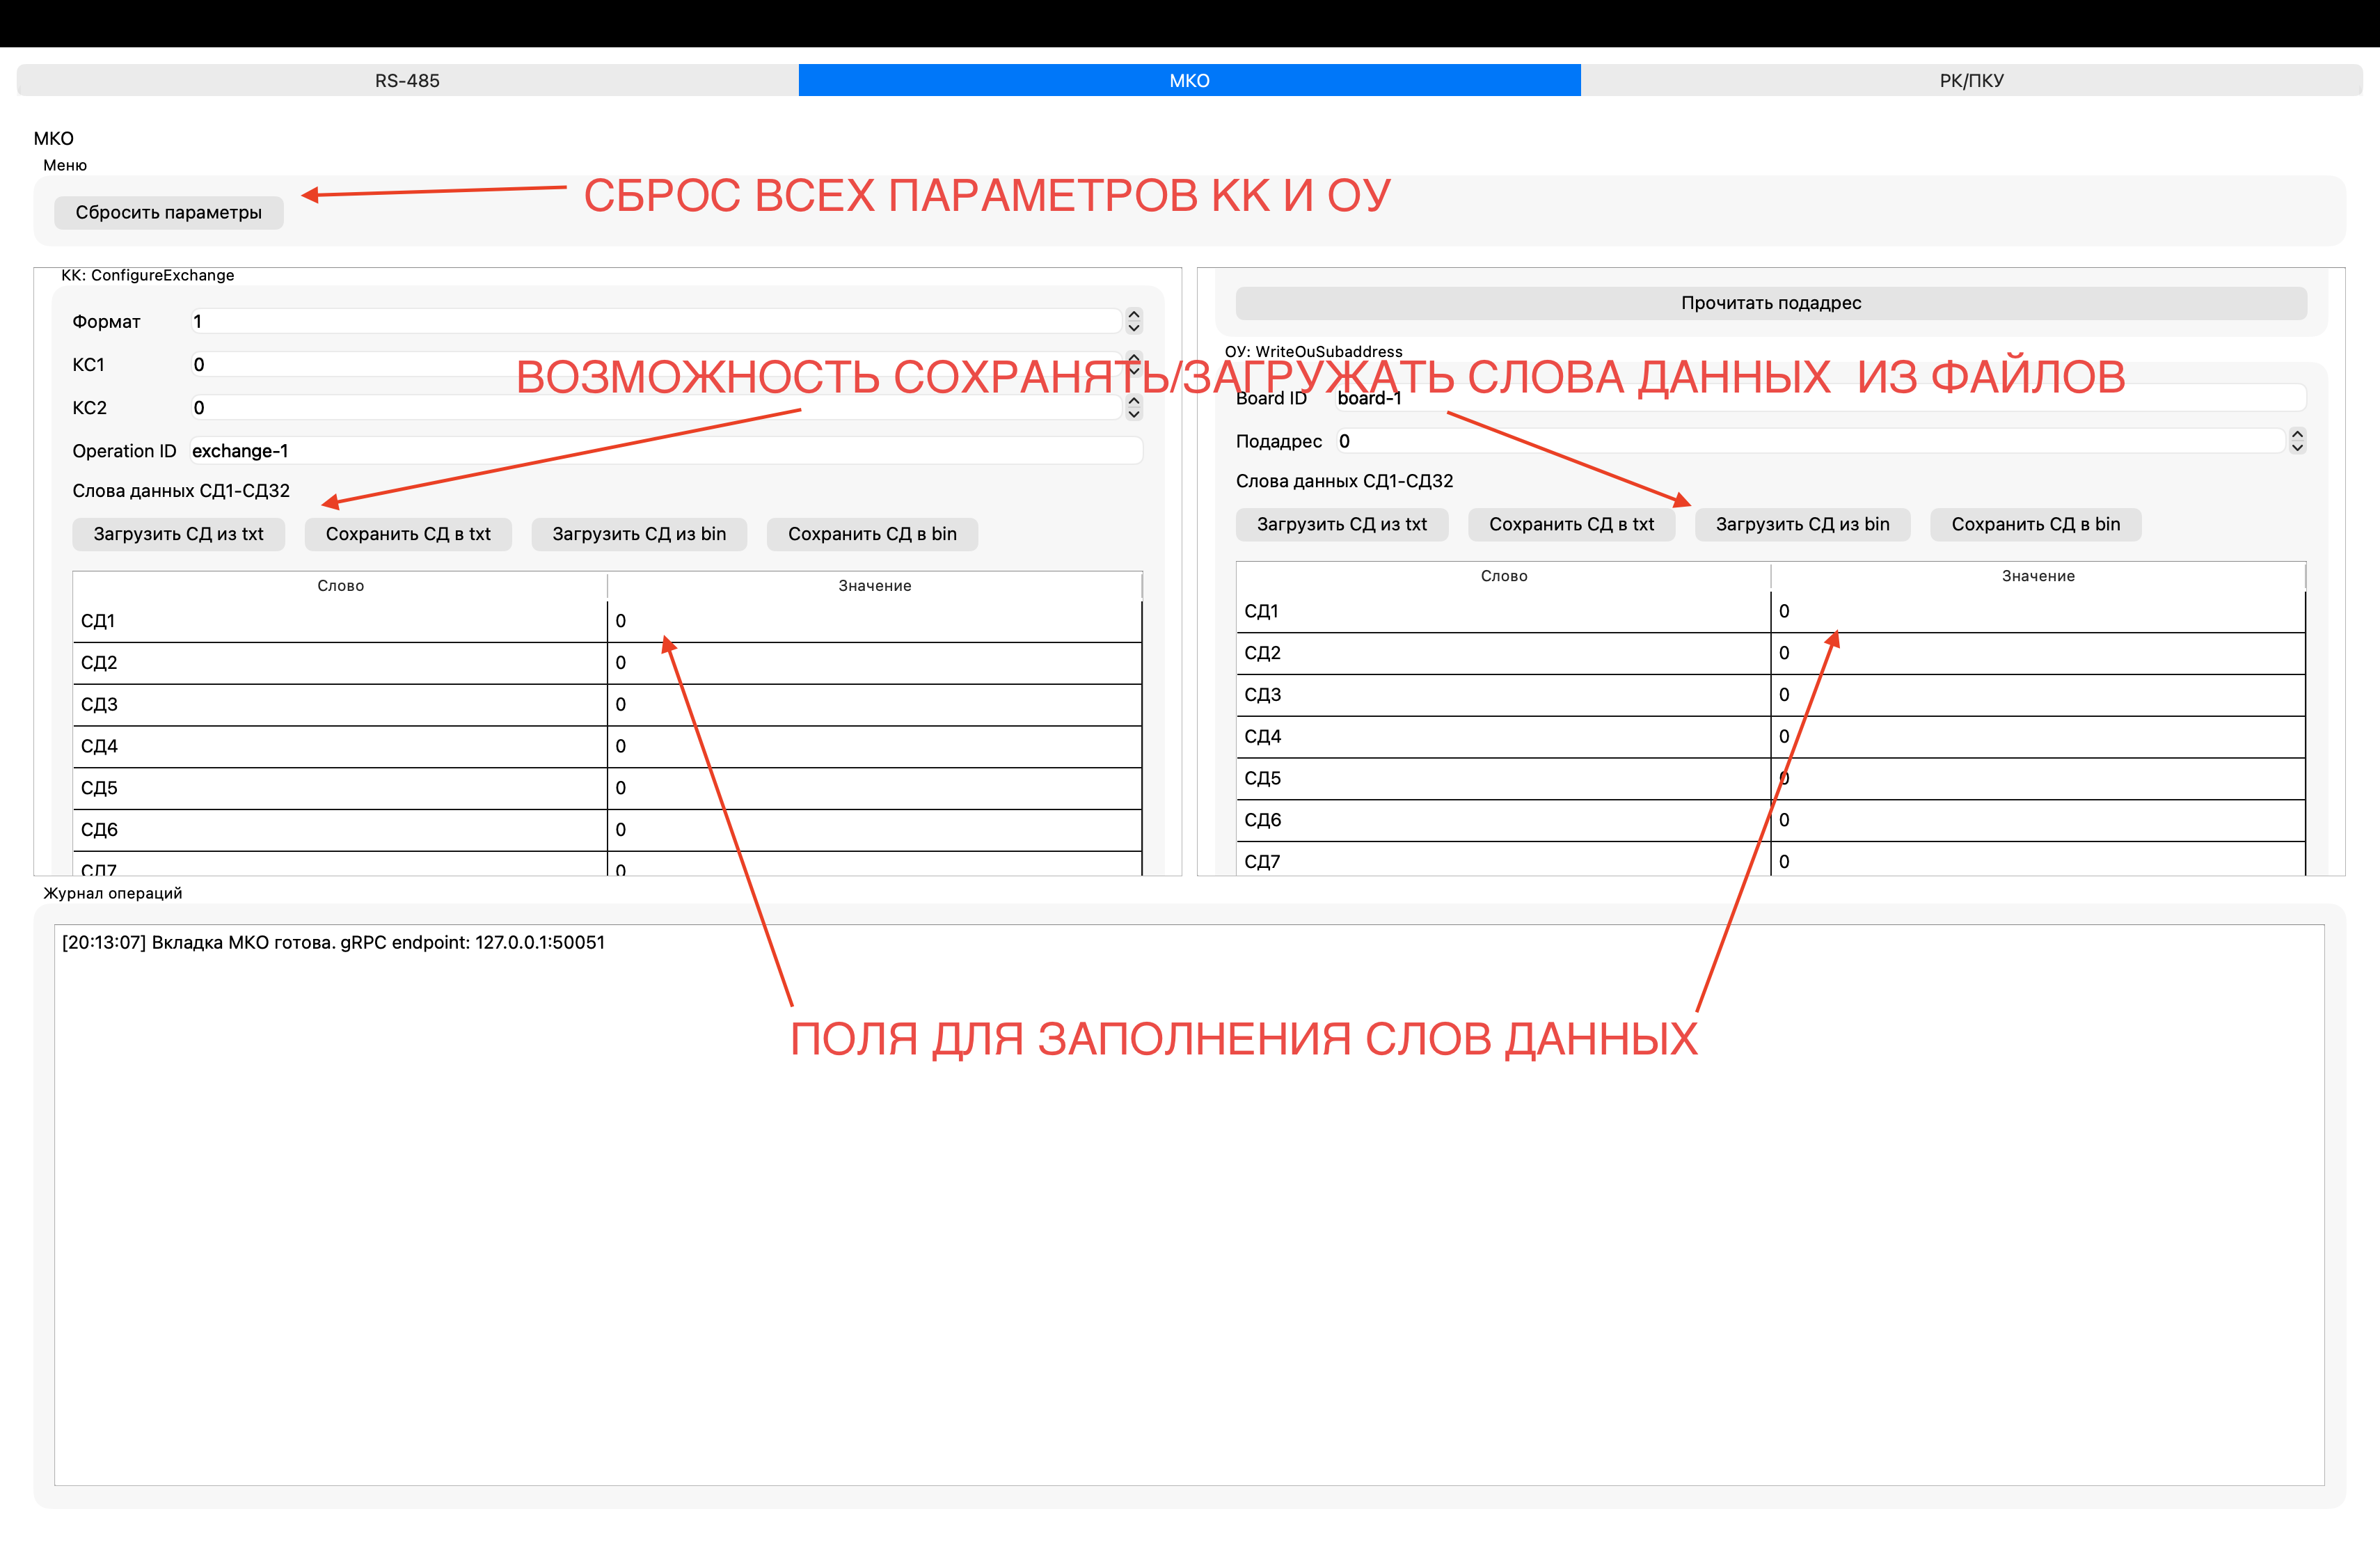
\includegraphics[width=\textwidth]{mko/image-2.png}
	\caption{Подсказки для ввода слов данных}
\end{figure}

\begin{table}[H]
	\caption{Диапазоны значений вкладки МКО}
	\begin{tabularx}{\textwidth}{|p{0.30\textwidth}|p{0.20\textwidth}|X|}
		\hline
		\textbf{Поле} & \textbf{Диапазон} & \textbf{Пояснение} \\
		\hline
		Номер МКО & 1--2 & Один номер МКО не должен одновременно использоваться в режиме КК и режиме ОУ. Интерфейс автоматически разводит выбранные номера. \\
		\hline
		Канал & 0--1 & 0 --- основной канал, 1 --- резервный канал. \\
		\hline
		\texttt{bus\_control} & 0--1 & Поле управления шиной для настройки КК. \\
		\hline
		Адрес ОУ & 0--30 & Адрес оконечного устройства. \\
		\hline
		Подадрес ОУ & 0--30 & Подадрес области приема или передачи ОУ. \\
		\hline
		Ответное слово, векторное слово, слово самотеста & 0--65535 & Значения являются 16-битными словами. Рекомендуется вводить их в шестнадцатеричном виде. \\
		\hline
		КС1, КС2 & 0--65535 & Командные слова обмена КК. \\
		\hline
		СД1--СД32 & 0--65535 & Слова данных МКО. Интерфейс технически читает \texttt{uint32}, но для корректного слова МКО следует использовать 16-битный диапазон. \\
		\hline
		Формат обмена & 1, 2, 4, 5, 6, 7, 9, 10 & Поддерживаемые драйвером форматы обмена КК. Для каждого формата драйвер дополнительно проверяет допустимое количество слов данных. \\
		\hline
		Remote port & 1--65535 & UDP-порт платы МКО. \\
		\hline
	\end{tabularx}
\end{table}

\subsubsection{Порядок начала работы}

После запуска основной программы оператор открывает вкладку МКО и проверяет, что в журнале операций появилось сообщение о готовности вкладки и адресе gRPC endpoint. Далее оператор выбирает требуемый режим работы: КК или ОУ.

Один и тот же номер МКО не должен одновременно использоваться в двух режимах. При совпадении номеров интерфейс автоматически изменяет один из выбранных номеров и выводит предупреждение в журнал.

\subsubsection{Работа в режиме КК}

В режиме КК оператор настраивает контроллер канала, задает обмен и запускает его выполнение.

Блок ``КК: ConfigureKK'' настраивает плату МКО в режиме контроллера канала. Оператор задает идентификатор платы, номер МКО, канал, параметры управления шиной, адрес ОУ, служебные слова и адрес платы МКО.

Кнопка ``Настроить КК'' выполняет gRPC-вызов \texttt{ConfigureKK}. В журнал операций выводятся параметры вызова и результат: успешное выполнение либо текст ошибки.

Блок ``КК: ConfigureExchange'' задает параметры обмена: формат, командные слова КС1 и КС2, идентификатор операции и массив слов данных СД1--СД32.

Перед таблицей СД расположены кнопки:

\begin{itemize}
	\item ``Загрузить СД из txt'' --- заполняет таблицу из текстового файла;
	\item ``Сохранить СД в txt'' --- сохраняет текущие значения таблицы в текстовый файл;
	\item ``Загрузить СД из bin'' --- заполняет таблицу из двоичного файла;
	\item ``Сохранить СД в bin'' --- сохраняет текущие значения таблицы в двоичный файл.
\end{itemize}

Кнопка ``Настроить обмен'' выполняет gRPC-вызов \texttt{ConfigureExchange}. В журнал выводятся \texttt{board\_id}, формат, КС1, КС2 и результат выполнения.

Кнопка ``RUN: запустить обмен'' выполняет gRPC-вызов \texttt{RunExchange}. Этот вызов отправляет команду запуска обмена в драйвер. В журнал выводятся \texttt{board\_id}, \texttt{operation\_id} и результат выполнения.

Кнопка ``Подписаться на результаты'' открывает получение результатов обмена КК через поток \texttt{SubscribeExchangeResults}. После открытия подписки результаты обмена отображаются в журнале операций. Для прекращения получения данных оператор повторно использует кнопку подписки, если в интерфейсе она перешла в режим отписки, либо завершает работу вкладки.

\subsubsection{Работа в режиме ОУ}

В режиме ОУ оператор настраивает оконечное устройство, читает и записывает подадреса, меняет ответное слово и контролирует входящие команды.

Блок ``ОУ: ConfigureOu'' настраивает плату в режиме оконечного устройства. Оператор задает идентификатор платы, номер МКО, канал, адрес ОУ, ответное слово и адрес платы.

Кнопка ``Настроить ОУ'' выполняет gRPC-вызов \texttt{ConfigureOu}. В журнал выводятся основные параметры настройки и результат выполнения.

Блок ``ОУ: SubscribeOuCommands'' открывает подписку на входящие команды ОУ. Оператор задает \texttt{board\_id} и нажимает ``Подписаться на команды ОУ''. После открытия подписки кнопка меняет назначение на отписку.

При получении события из потока \texttt{SubscribeOuCommands} в журнал выводятся командное слово, слово результата, направление обмена, адрес ОУ, подадрес, количество слов, расшифровка команды и расшифровка результата.

Блок ``ОУ: ReadOuSubaddress'' читает выбранный подадрес ОУ. Оператор задает \texttt{board\_id}, номер подадреса и выбирает область: область приема или область передачи.

Кнопка ``Прочитать подадрес'' выполняет gRPC-вызов \texttt{ReadOuSubaddress}. В журнал операций выводится структура ответа: подадрес, командное слово, слово результата, расшифровка результата и массив СД.

Блок ``ОУ: WriteOuSubaddress'' записывает слова данных в область передачи выбранного подадреса ОУ. Оператор задает \texttt{board\_id}, подадрес и значения СД1--СД32.

Перед таблицей СД доступны кнопки загрузки и сохранения в текстовом и двоичном формате. Кнопка ``Записать подадрес'' выполняет gRPC-вызов \texttt{WriteOuSubaddress}. В журнал выводятся \texttt{board\_id}, подадрес и переданный массив СД.

Блок ``ОУ: SendRawOuData'' предназначен для отправки сырых слов данных ОУ. Поля и файловые операции аналогичны блоку \texttt{WriteOuSubaddress}.

Кнопка ``Отправить сырые данные ОУ'' выполняет gRPC-вызов \texttt{SendRawOuData}. В журнал выводятся \texttt{board\_id}, подадрес и массив переданных слов.

Блок ``ОУ: SetOuResponseWord'' изменяет ответное слово ОУ. Оператор задает идентификатор платы, номер МКО, канал, адрес ОУ и новое ответное слово.

Кнопка ``Установить ответное слово'' выполняет gRPC-вызов \texttt{SetOuResponseWord}. В журнал выводятся параметры вызова и результат выполнения.

Блоки ``ОУ: ClearReceiveBuffer'' и ``ОУ: ClearTransmitBuffer'' очищают соответственно буфер приема и буфер передачи для выбранной платы и номера МКО.

Кнопки ``Очистить буфер приема'' и ``Очистить буфер передачи'' выполняют gRPC-вызовы \texttt{ClearReceiveBuffer} и \texttt{ClearTransmitBuffer}. В журнал выводятся \texttt{board\_id}, номер МКО и результат операции.

\subsubsection{Завершение работы вкладки МКО}

Перед завершением работы оператор прекращает активные подписки на результаты обмена и входящие команды ОУ, если они были открыты. После этого можно закрыть графический интерфейс. При локальной отладке затем завершаются микросервис МКО и заглушка драйвера.
